    \p
    دنباله را روی یک خط تصویر می‌کنیم، به طوری که هر نقطه نشان‌دهنده‌ی یک عدد باشد. یک عضو دل‌خواه، به طور مثال $m$-امین عدد را انتخاب می‌کنیم.
    حال دو زیردنباله از دنباله اصلی مانند
    $L_m$
    و
    $R_m$
   را طوری می‌سازیم که 
    $L_m$
   بزرگ‌ترین زیر‌دنباله‌ی اکیدا صعودی باشد که به $m$-امین عضو دنباله ختم شده و 
   $R_m$
   بزرگ‌ترین زیر‌دنباله‌ی اکیدا نزولی باشد که از عضو $m$-ام دنباله شروع می‌شود. 
\begin{center}
    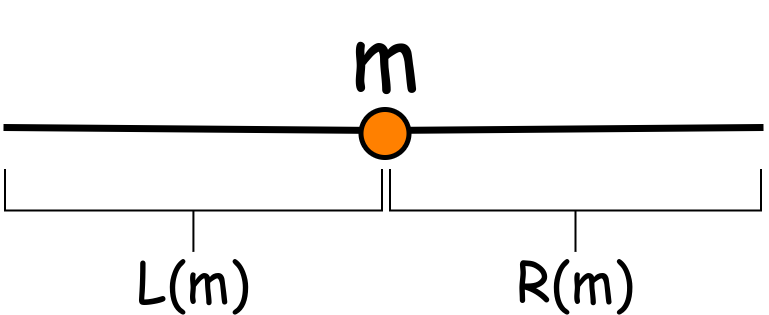
\includegraphics[width=3.5cm]{1.png}
\end{center}
\p
   حال اثبات می‌کنیم به ازای هر
     $m$
     جدید، زوج مرتب متمایزی از زیرمجموعه‌های
     $L_m$
     و
     $R_m$
      به‌دست می‌آید. $k$-امین عدد را در نظر می‌گیریم، به طوری که با $m$-امین عدد مساوی نبوده و
      $m < k$ 
      باشد، یعنی $m$-امین عضو سمت چپ $k$-امین عضو
      قرار داشته باشد. حال اگر مقدار $m$-امین عضو بیش‌تر از $k$-امین عضو باشد، 
      $R_m$
      حداقل یک عضو بیش‌تر از
      $R_k$
      دارد (در اشکال، محور افقی نمایش‌گر اعضای دنباله و محور عمودی نشان‌دهنده‌ی مقادیر هر یک می‌باشند): 
\begin{center}
    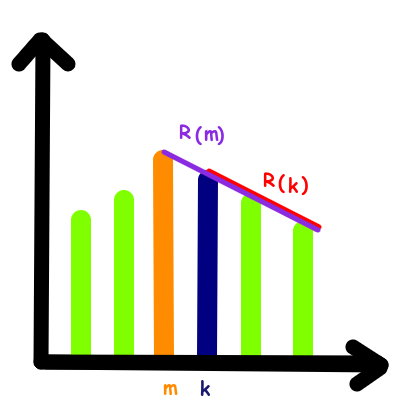
\includegraphics[height=4cm]{2.png}
\end{center}
\p
      پس زوج‌های
    $(L_{m}, R_{m})$
    و
    $(L_{k}, R_{k})$
با هم متمایز هستند. در حالتی که مقدار $m$-امین عضو کم‌تر از $k$-امین عضو باشد،
   $L_k$
      حداقل یک عضو بیش‌تر از
      $L_m$
      داشته و تمایز زوج‌های
    $(L_{m}, R_{m})$
    و
    $(L_{k}, R_{k})$
اثبات می‌شود:
\begin{center}
    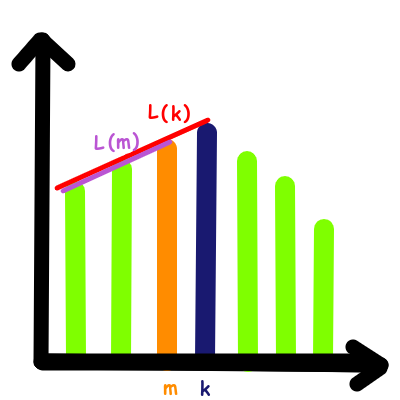
\includegraphics[height=4cm]{3.png}
\end{center}
\p
 در حالت 
    $m > k$
                نیز  به همین صورت، عکس این نتایج رخ می‌دهد. بنابراین ثابت کردیم تمام زوج‌های
    $(L_{m}, R_{m})$
    به ازای $m$های مختلف، متمایز هستند. 
    \p
    حال برای اثبات حکم با استفاده از برهان خلف، فرض می‌کنیم زیر دنباله‌ای اکیدا صعودی به طول 
    $p+1$
      یا زیردنباله‌ای اکیدا نزولی به طول 
    $q+1$
      موجود نباشد. بنابراین: 
    $$1\leq |L_{m}|\leq p$$
      و 
    $$1\leq |R_{m}|\leq q$$
    پس برای هر $m$، زوج 
    $(L_{m}, R_{m})$
      می‌تواند 
    $p \times q$
    حالت داشته باشد و از آن‌جایی که $m$ می‌تواند 
    $pq + 1$
      مقدار مختلف داشته باشد، طبق اصل لانه‌ی کبوتری، حداقل 
      $2$
       زوج 
    $(L_{m}, R_{m})$
      با هم برابر بوده که با متمایز بودن همه‌ی زوج‌های 
    $(L_{m}, R_{m})$
      در تناقض است. بنابراین فرض خلف نادرست است و درستی حکم ثابت می‌شود. 